\begin{center}
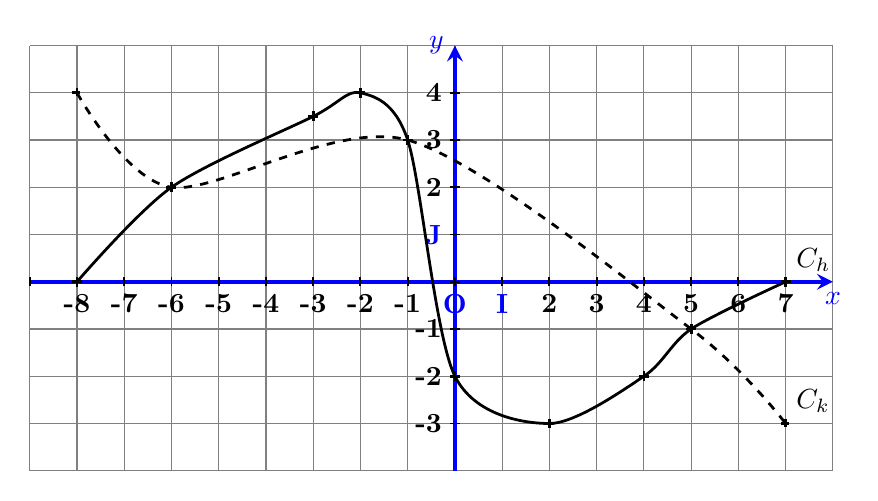
\begin{tikzpicture}[scale=0.6,>=stealth]
            \draw[gray] (-9,-4)grid(8,5);
            \draw[->,line width=1.5pt,color=blue] (-9,0)--(8,0)node[below] {$x$};
            \foreach \x in {-8,-7,-6,-5,-4,-3,-2,-1,2,3,4,5,6,7}
\draw[color=black] (\x,2pt) -- (\x,-2pt) node[below,font=\bfseries] {\x};
            \draw[->,line width=1.5pt,color=blue] (0,-4)--(0,5)node[left] {$y$};
            \foreach \y in {-3,-2,-1,2,3,4}
\draw[color=black] (2pt,\y) -- (-2pt,\y) node[left,font=\bfseries] {\y};
            \coordinate (O) at (0,-2pt); \draw (O) node[below,font=\bfseries,color=blue] {O};
            \coordinate (I) at (1,-2pt); \draw (I) node[below,font=\bfseries,color=blue] {I}; 
            \foreach \x in {-9,...,7}  
            \draw[line width=0.7pt] (\x,-0.1)--(\x,0.1);
            \coordinate (J) at (-2pt,1); \draw (J) node[left,font=\bfseries,color=blue] {J}; 
            \foreach \x in {-3,...,4} 
            \draw[line width=0.7pt] (-0.1,\x)--(0.1,\x);
            \draw[line width=1pt] plot[smooth=200,mark=+,mark options={scale =1.5}] 
            coordinates{(-8,0)(-6,2)(-3,3.5)(-2,4)(-1,3)(0,-2)(2,-3)(4,-2)(5,-1)(7,0)} 
            node[above right]{$\calig C_h$};
            \draw[dashed, line width=1pt] plot[smooth=200,mark=+,mark options={scale =1.5}] 
            coordinates{(-8,4)(-6,2)(-1,3)(5,-1)(7,-3)} node[above right]{$\calig C_k$};
\end{tikzpicture}
\end{center}